\chapter{Range-clone}
\label{chap:clone}

This chapter describes another \bet operation, range-clone, which can be used
to implement file or directory clones and renames on full-path-indexed \betrfs.
Unlikely a range-rename, which completes all its work at once, a range-clone
injects a new type of message, the \goto messages, to the \bet.
The \bet then flushes \goto messages with other messages in batches, gradually
finishing the range-clone works.
Therefore, range-clone fits into the write-optimized framework of \bets.

This chapter first describes the range-clone interface,
followed by how range-clones are implemented on \bets.
At last, this chapter describes a new technique, preferential splitting, which
makes range-clones more efficient.

\section{The range-clone interface}

\begin{table}[t]
    \centering
    \begin{tabular}{c | l}
        \hline
        Type of File System Operation & Key/Value Store Operations \\
        \hline
        \hline
        File Rename & \mdb$\rightarrow$put(\textit{dst}); \\
                    & \mdb$\rightarrow$del(\textit{src}); \\
                    & \ddb$\rightarrow$range-clone(\textit{src}, \textit{dst}, true); \\
        \hline
        Directory Rename & \mdb$\rightarrow$put(\textit{dst}); \\
                         & \mdb$\rightarrow$del(\textit{src}); \\
                         & \mdb$\rightarrow$range-clone(\textit{src/}, \textit{dst/}, true); \\
                         & \ddb$\rightarrow$range-clone(\textit{src/}, \textit{dst/}, true); \\
        \hline
        File Clone  & \mdb$\rightarrow$put(\textit{dst}); \\
                    & \ddb$\rightarrow$range-clone(\textit{src}, \textit{dst}, false); \\
        \hline
        Directory Clone  & \mdb$\rightarrow$put(\textit{dst}); \\
                         & \mdb$\rightarrow$range-clone(\textit{src/}, \textit{dst/}, false); \\
                         & \ddb$\rightarrow$range-clone(\textit{src/}, \textit{dst/}, false); \\
        \hline
    \end{tabular}
    \caption[File system renames and clones in \betrfs with range-clones]{\label{tab:fsrc}
        \betrfs renames or clones \textit{src} to \textit{dst} by calling range-clones.}
\end{table}

Similar to range-rename, range-clone is defined as:
range-clone(\spre, \dpre, \delold), where \delold is a boolean.
It does the following things:
\begin{itemize}
\item it deletes all destination key/value pairs from the key/value store;
\item then, for any source key/value pair $(k,v)$ in the key/value store,
it inserts a key/value pair $(k',v)$ to the key/value store,
where $k$ is the concatenation of \spre and some suffix $s$ and $k'$ is the
concatenation of \dpre and the same suffix $s$;
\item if \delold is true, it deletes all source key/value pairs from the
key/value store.
\end{itemize}
If \delold is true, range-clone is equivalent to range-rename;
otherwise, range-clone is range-rename without deleting source key/value pairs.
Therefore, as summarized in Table~\ref{tab:fsrc},
file or directory renames on full-path-indexed \betrfs can be done
with range-clones just as they are done with range-renames.
And clones on full-path-index \betrfs are done in the similar ways with \delold
set to false.

\section{The range-clone operation}

This section shows the implementation of range-clone operations.
Because deleting source key/value pairs can be done by injecting a range-delete
message into the root node,
\delold is set to false throughout the section.

This section first shows all the changes needed if performing all operations
at the time of the range-clone, that is, all operations are on the critical
path, and mutual exclusion on the tree.
Then, this section shows how to enhance the design to minimize the critical
path, reduce locking, and move as much work as possible to the background.
Moving work to the background also reduce the total amount of CPU and IO work,
since \bets are designed to buffer changes and to schedule them IO-efficiently.

\subsection{Range-clone, on the critical path}

\begin{figure}
    \begin{subfigure}{\textwidth}
        \centering
        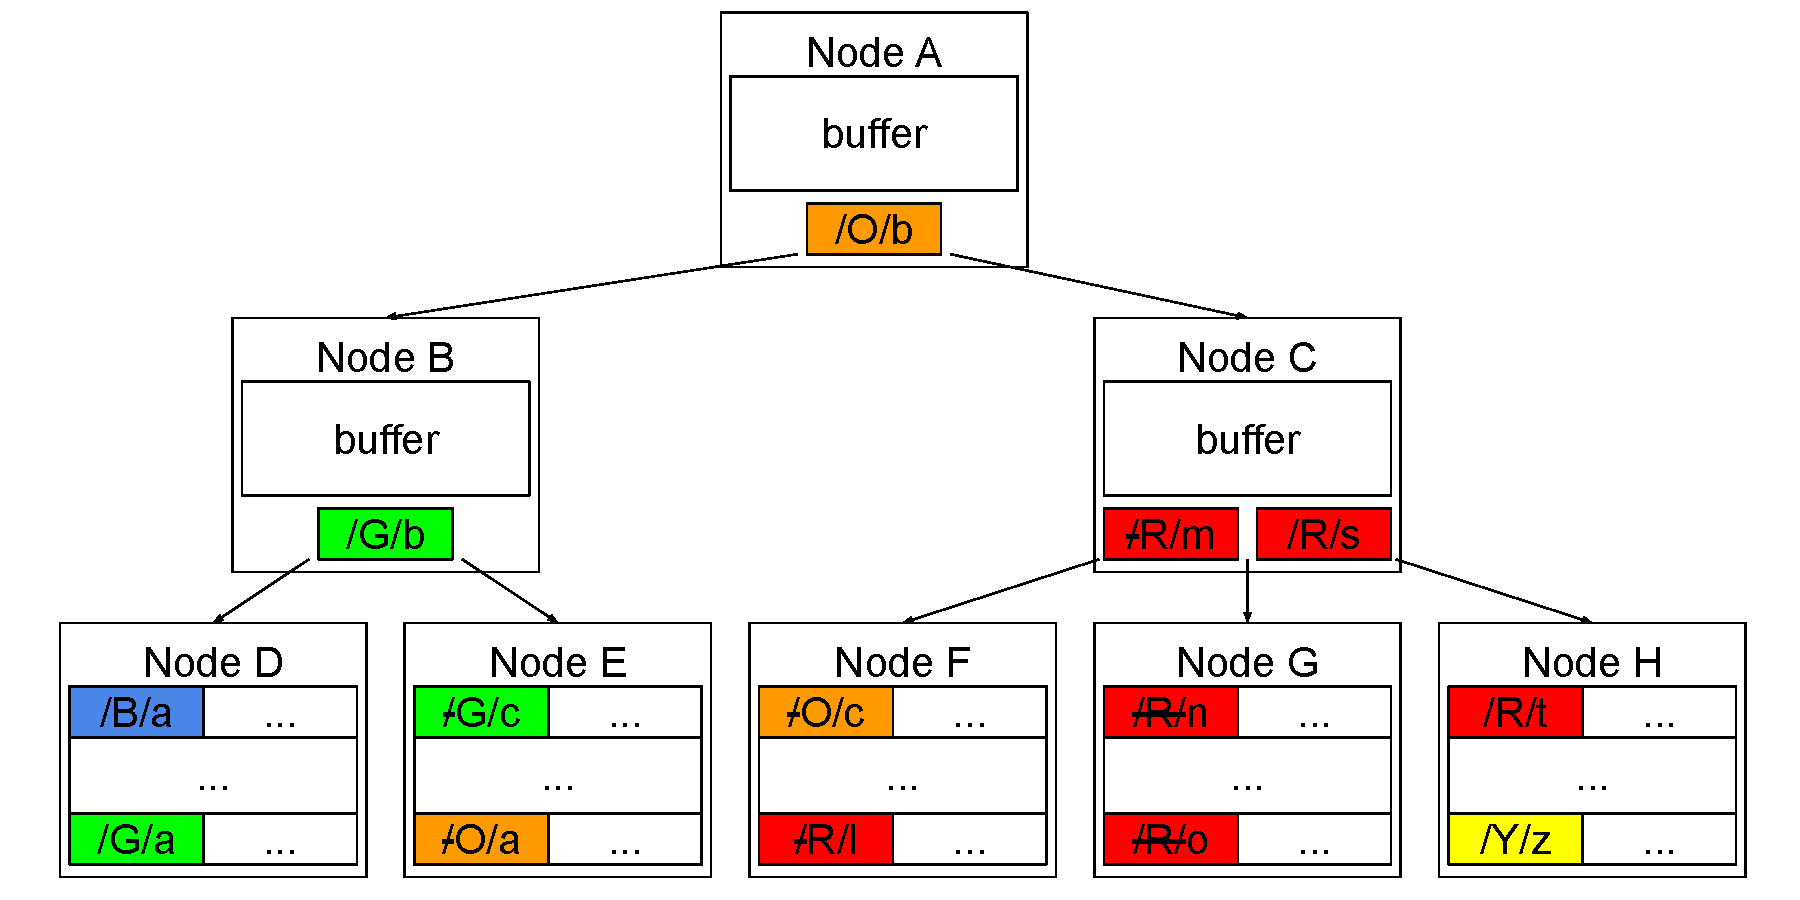
\includegraphics[width=.7\linewidth]{fig/rr-1}
        \caption{\label{subfig:rc-1} The \bet before the range-clone.}
    \end{subfigure}
    \begin{subfigure}{\textwidth}
        \centering
        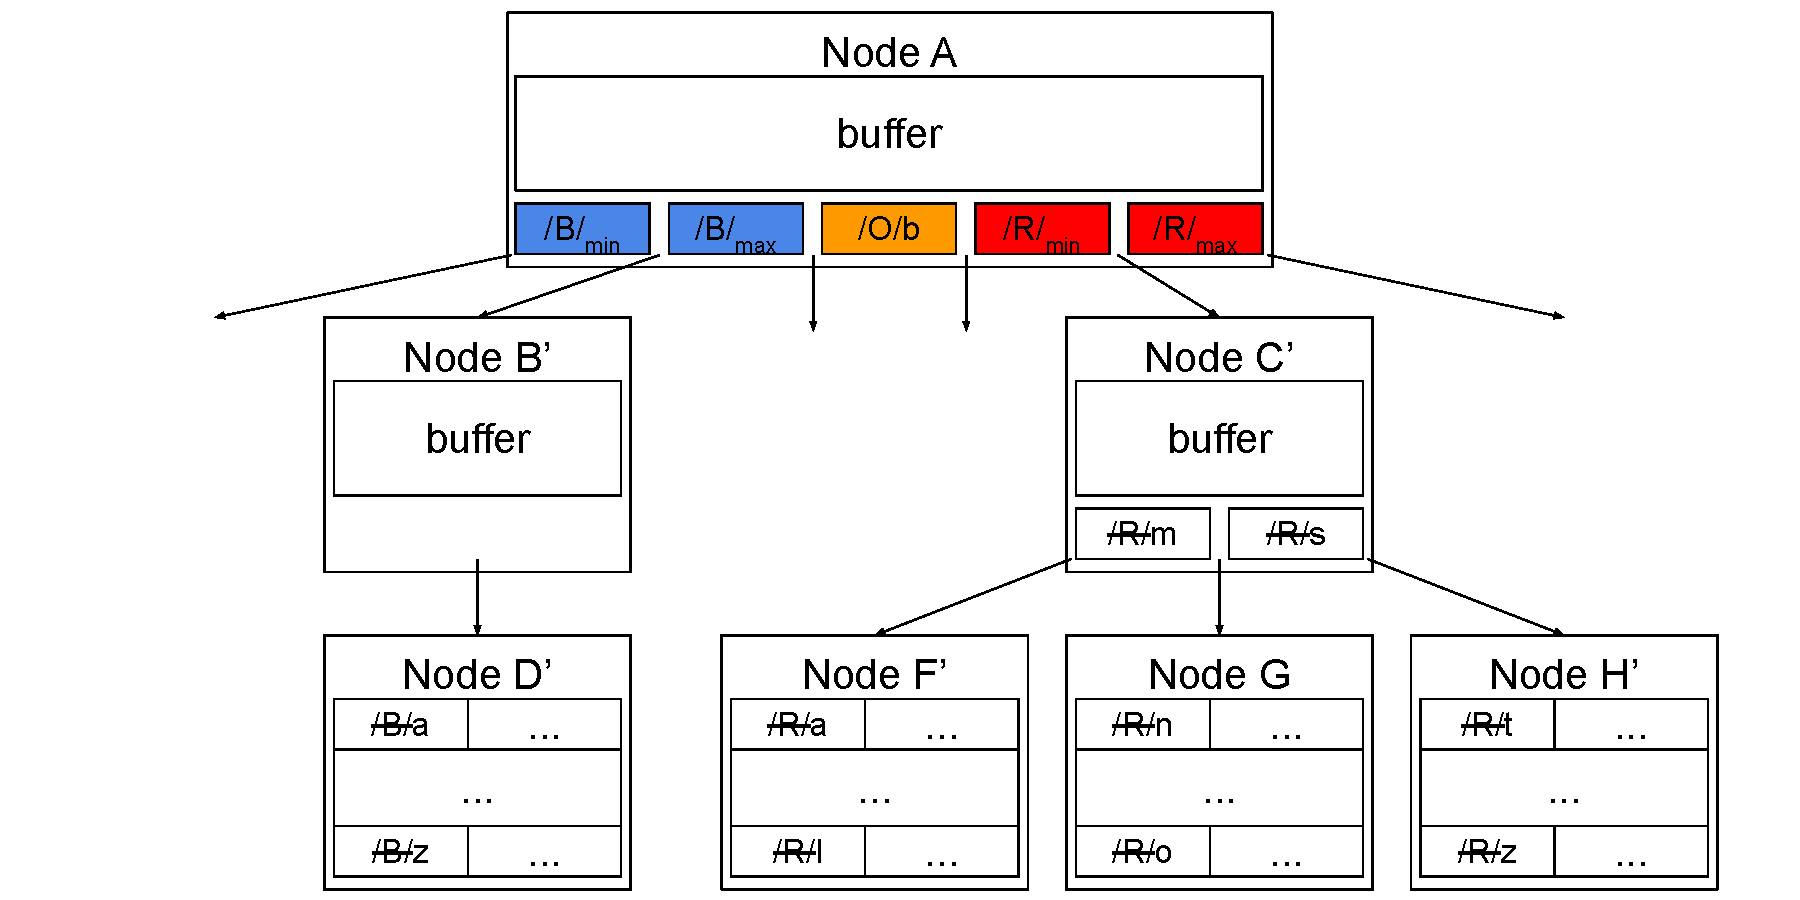
\includegraphics[width=.7\linewidth]{fig/rr-2}
        \caption{\label{subfig:rc-2} The range-clone slices out the source and
            destination subtrees.}
    \end{subfigure}
    \begin{subfigure}{\textwidth}
        \centering
        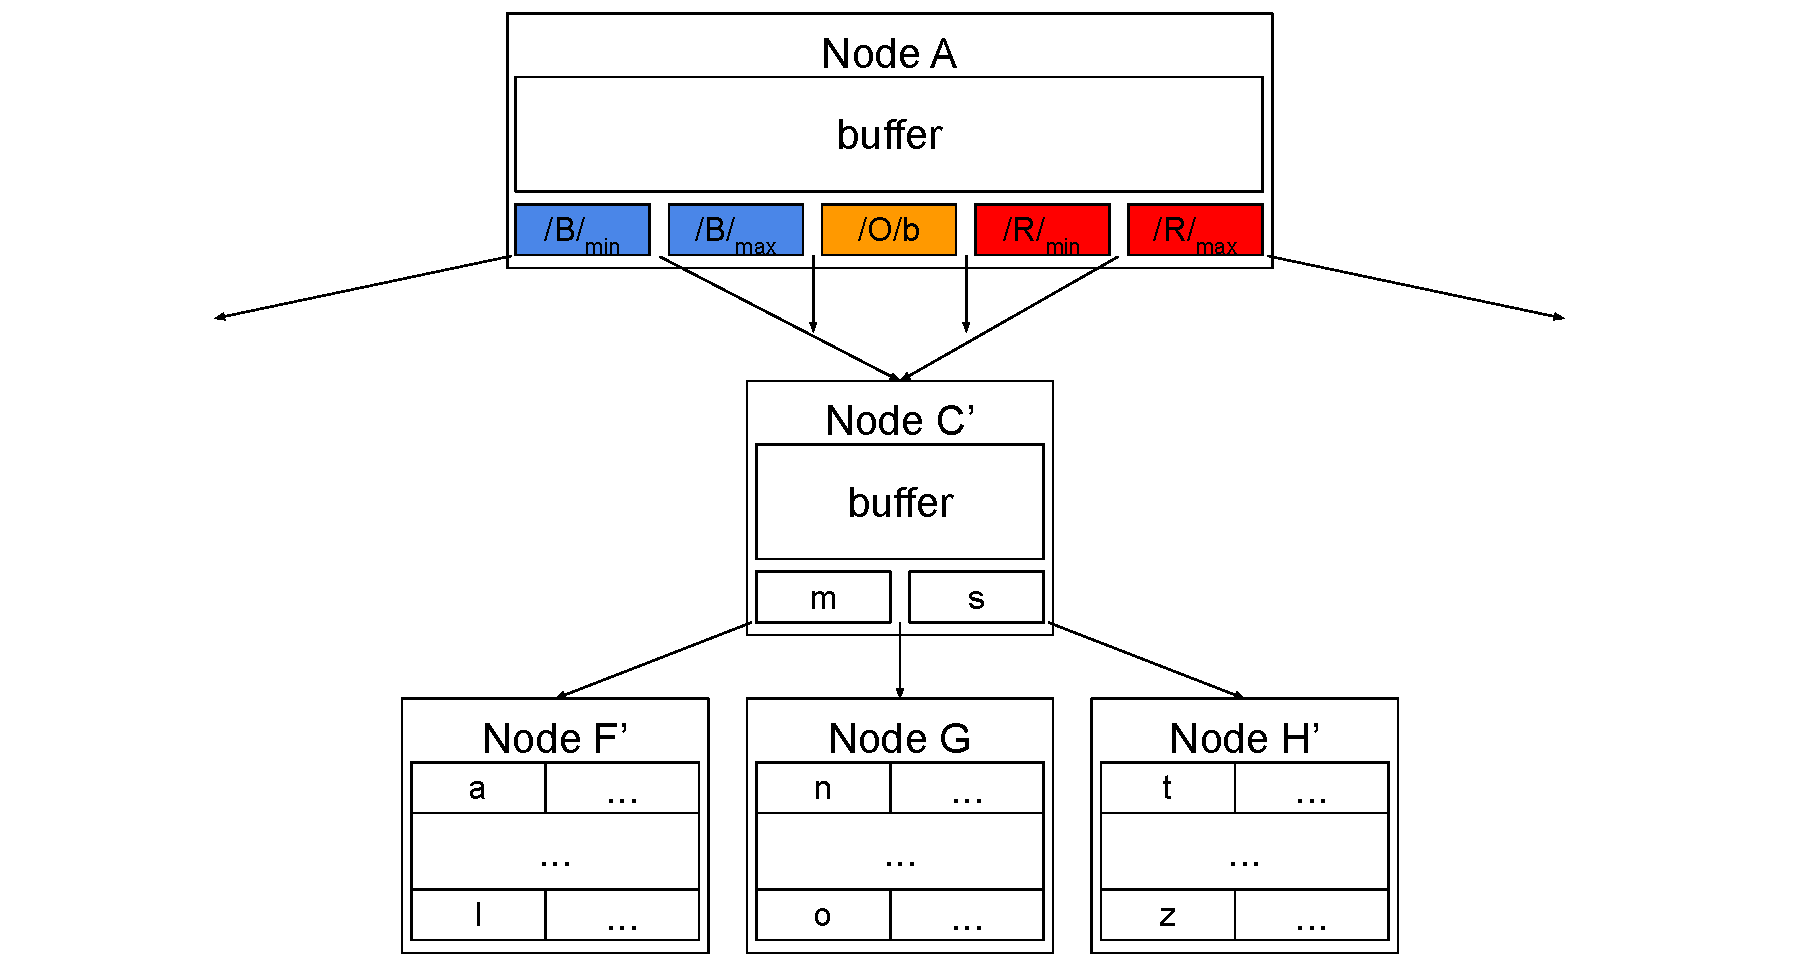
\includegraphics[width=.65\linewidth]{fig/rc-3}
        \caption{\label{subfig:rc-3} The range-clone discards the destination
            subtree and shares the source subtree.}
    \end{subfigure}
    \caption[All operations in range-clone]{\label{fig:rc}
        All operations needed in range-clone(``/R/'', ``/B/'').}
\end{figure}

The range-clone work can be done by slightly modifying the range-rename
operation.
In particular, after slicing out the source and destination subtrees with tree
surgery, range-rename swaps the two subtrees and injects a range-delete message
for source keys.
Instead, range-clone can share the source subtree in destination and send the
destination subtree to a background garbage collection thread.

Figure~\ref{fig:rc} shows the work of range-clone(``/R/'', ``/B/'') in the
lifted \bet in Figure~\ref{subfig:rc-1}.
Figure~\ref{subfig:rc-2} shows the lifted \bet after tree surgery, which slices
out the source and destination subtree.
The tree surgery here is identical to that in range-rename.
In Figure~\ref{subfig:rc-3}, the lifted \bet discards the destination subtree
rooted at Node $B'$, and set the parent-to-child pointer between ``/B/$_{min}$''
and ``/B/$_{max}$'' to Node $C'$, which is the root of the source subtree.

Range-rename transforms a lifted \bet into a lifted \bedag.
Because the DAG is generated by sharing subtrees in a tree,
there is still one root in the DAG,
which can reach all nodes in the DAG through parent-to-child pointers.
And since the source and destination subtrees generated by tree surgery are at
the same height, the length of any root-to-leaf path in the DAG is still
logarithmic in the size of the graph.

In a lifted \bedag, the root-to-leaf traversals of different queries may end up
reaching the same leaf node, fetching the same key/value pair.
However, because key lifting requires queries to reconstruct the full key by
concatenating lifted prefixes, different queries are able to see different keys.

\begin{figure}
    \begin{subfigure}{\textwidth}
        \centering
        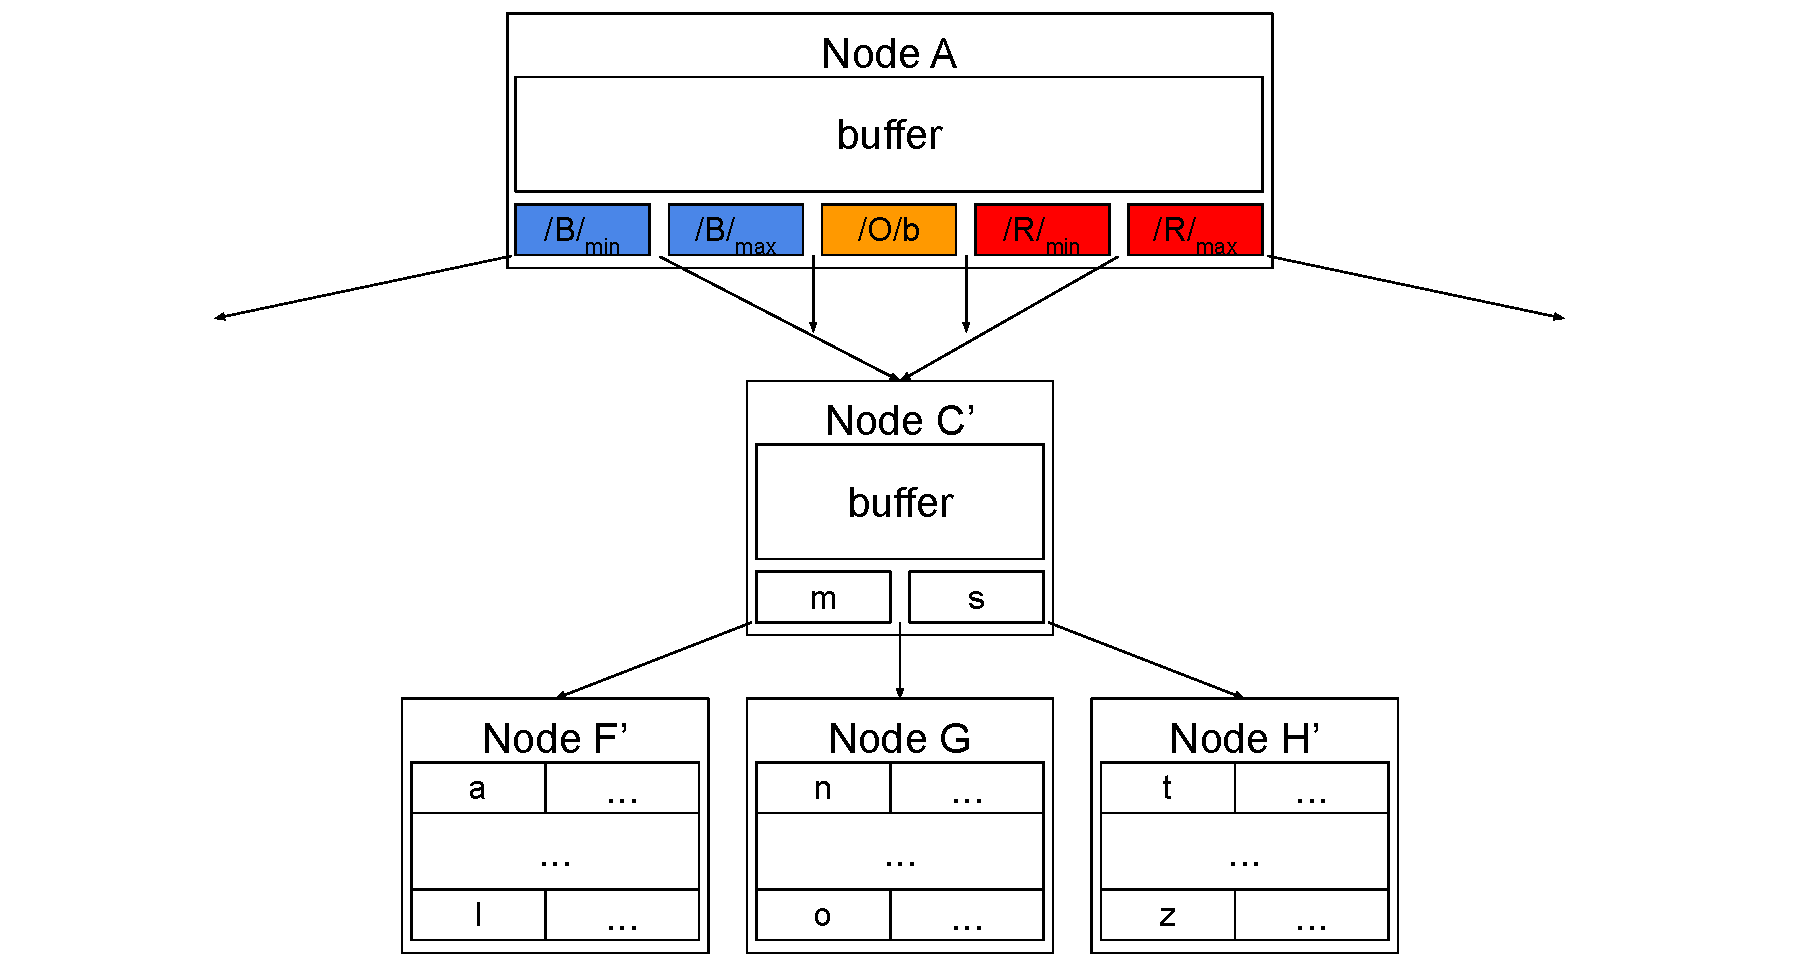
\includegraphics[width=.9\linewidth]{fig/rc-3}
        \caption{\label{subfig:cow-1} Node $C'$ is a shared by two
            parent-to-child pointers in Node $A$.}
    \end{subfigure}
    \begin{subfigure}{\textwidth}
        \centering
        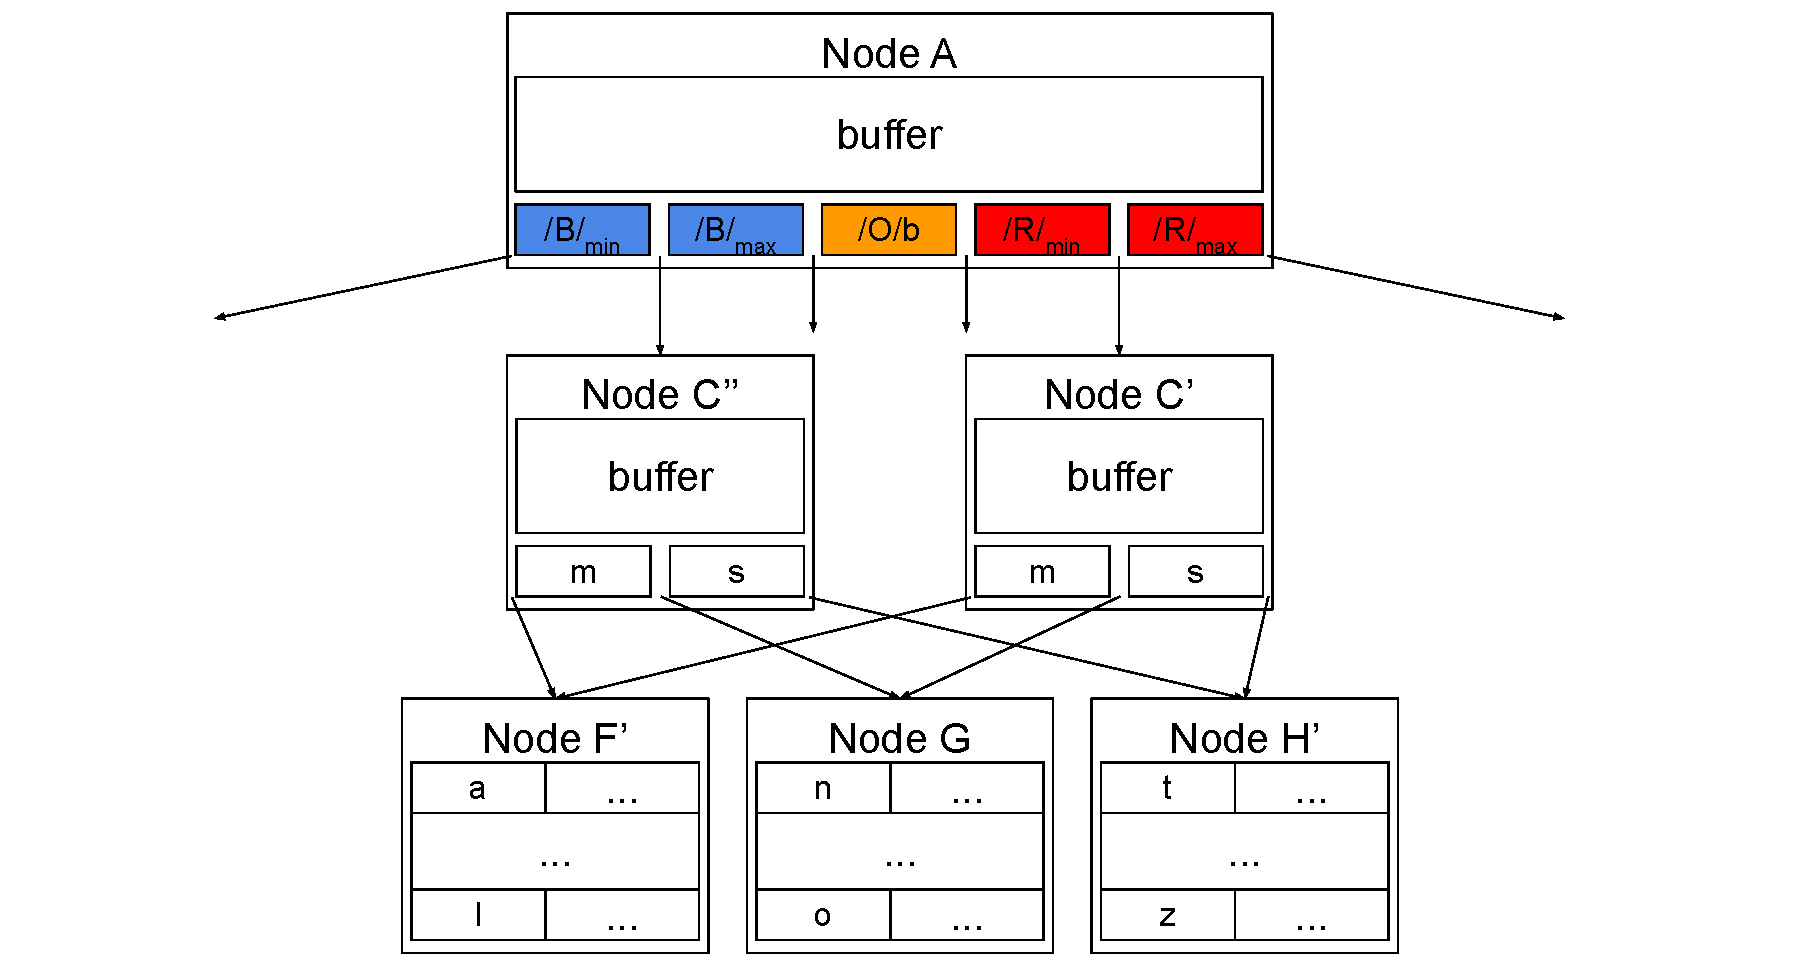
\includegraphics[width=.9\linewidth]{fig/cow-2}
        \caption{\label{subfig:cow-2} Before Node $A$ flushes ``/B/'' messages,
            it breaks the sharing creating Node $C''$, which is a clone of Node
            $C'$.}
    \end{subfigure}
    \caption[\bedags break node sharing with CoW]{\label{fig:cow}
        When the parent accumulates enough messages to flush to a shared node,
        it breaks the sharing with Cow.}
\end{figure}

Any writes to a shared node must first break the sharing of the node, the
\bedag maintains reference counting for each node to track the sharing status of
nodes.
In particular, \fti has a node table that maps node IDs to physical locations on
disk.
The \bedag stores the reference count of each node in the node table alongside
the mapping.
Before writing to a node, the \bedag must check the reference count of the node.

The \bedag breaks the sharing of a node using Copy-on-Write (CoW).
After range-rename, one parent of the shared node might choose to flush its
messages to the node.
At this moment, the lifted \bedag creates a new node that is identical to the
shared node, sharing all children of the node.
The lifted \bedag then sets the parent-to-child pointer to the new node and
performs the flush.

Figure~\ref{fig:cow} shows an example of the CoW process.
In Figure~\ref{subfig:cow-1}, Node $A$ has two parent-to-child pointers to
Node $C'$ with reference count 2.
Note, Node $F'$, $G$ and $H'$ have reference count 1.
When Node $A$ accumulates enough messages and wants to flush messages with
``/B/'', it clones Node $C'$ to break the sharing.
As shown in Figure~\ref{subfig:cow-2}, the \bedag creates a new Node $C''$
identical to Node $C'$.
Now, both Node $C'$ and $C''$ have reference count, while Node $F'$, $G$ and
$H'$ have reference count 2.

\subsection{\goto messages}

The implementation of range-clone with \goto messages delays the tree surgery
work to the flushes in the lifted \bedag.
This design puts the tree surgery in the write-optimized framework of the data
structure.

\section{Preferential splitting}

Most of the additional background work in range-clone is about removing
unrelated keys and unlifted prefix data from fringe nodes, which
contain both cloned and non-cloned data.
Therefore, it is beneficial to reduce the number of fringe nodes.

The baseline \bet splits nodes evenly.
When a leaf needs to be split, the middle key is picked as the new piovt
separating the two new leaves to be generated.
A non-leaf node split can be viewed as promoting the middle pivot in the node to
the parent.

Preferential splitting generates pivots that maximizes the common prefix under
the leaf, subject to the constraint that both leaves should be at least 1/4
full.
This strategy reduces the likelihood of having fringe nodes
in a range-clone and bounds the how unbalanced leaves can be.

A naive approach would compare all keys in the range of [1/4, 3/4] of the leaf
and picking the pair of two adjacent keys that share the shortest common prefix.
But this scan can be costly.

Preferential splitting only requires the reading of two keys.
Because the shortest common prefix of adjacent keys is the same as the common
prefix of the smallest (at 1/4 of the leaf) candidate key, $k_{s}$ and
the largest (at 3/4 of the leaf) candidate key, $k_{l}$,
a good pivot can be constructed from these two keys.
In particular, preferential splitting generates a pivot that is maximum key with
prefix $p_{s}$, where $p_{s}$ that is the shortest prefix of $k_{s}$ that
contains the LCP of $k_{s}$ and $k_{l}$ and has a slash or a end-of-string as
the last character.

\section{Summary}
